\chapter{Testing \& Evaluation}\label{ch:TestAndEval}
This chapter evaluates the overall project and provides results of testing.

\section{Testing}
\subsection{Unit Testing}
Unit testing is the practice of testing different elements of the software automatically, using a test program to provide inputs to each element and evaluate the outputs.
The tests are usually written before or at the same time as the tested componenents. According to Miguel Grindberg \citep{book:Grindberg2014FlaskWebDevelopment}, "There are two very good reasons for writing unit tests. When implementing new functionality, unit tests are used to confirm that the new code is working in the expected way. ... A second, more important reason is that each time the application is modified, all the unit tests built around it can be executed to ensure that there are no regressions  in the existing code; in other words, that the new changes did not affect the way the older code works." In a way, tests provide a safety net, meaning you can refactor the code at any time without the risk of breaking the original functionality. 

Due to the time constraints, the focus was on testing only for the critical parts of the project functionality. For this project it was especially important to ensure good code coverage for the business logic behind the model layer (prediction feature) and the external service layer of the application (api wrapper) explained in the chapter "Implementation" \ref{ch:Implementation}, section "Application Architecture". SureThing has a suite of 30 unit tests that can be run anytime to validate this part of the application functionality. Tests in this project are performed using Python \emph{unittest} library. 

\subsection{Continuous Integration with Travis CI}
As the application grows, it may become to take too long to run the unit tests. Therefore, it is worth automating this process by setting up a "Continuous Integration" or CI server. As a CI server was chosen Travis CI being easy to set up and available for free as a part of the GitHub Student Developer Pack. 
The service takes care of the unit testing allowing the developer to focus purely on the development process. Travis builds are triggered automatically when developer checks in the project code into the GitHub repository. Intergating Travis CI was just a matter of creation a configuration file \emph{travis.yml}. 

\begin{figure}[H]
	\begin{center}
		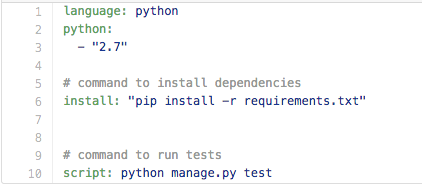
\includegraphics[width=.60\linewidth,natwidth=610,natheight=540]{eval/images/travisYml}
		\caption{Travis CI configuration file.} \label{fig:using:travisyml}
\end{center}
	
A Travis status icon indicating whether the tests passed or failed was embedded into the README file. This is a convinient feature that helped to keep an eye on the build status from the GitHub repository.

\end{figure}\begin{figure}[H]
	\begin{center}
		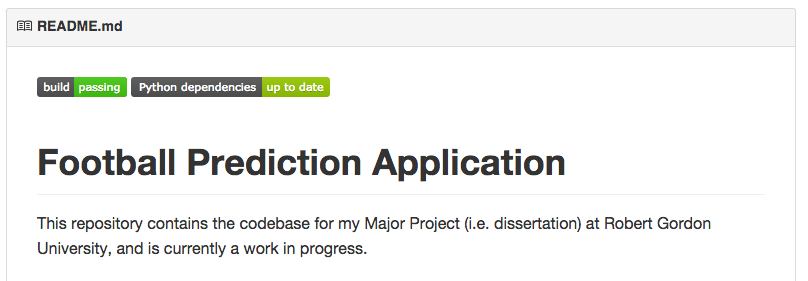
\includegraphics[width=.90\linewidth,natwidth=610,natheight=642]{eval/images/travisBadge}
		\caption{An extract from README on GitHub. Travis status icon indicates that the last build passed.} \label{fig:using:travisbadge}
	\end{center}
\end{figure}

\subsection{System Testing}
System Testing – This will test the system as a whole. This will be run by the developer taking into account the users requirements. Test cases will be created from the requirements with the inputs and expected outputs noted before the testing starts. Some of the test cases may satisfy more than one of the requirements. The tests will be carried out via the black box testing technique.

\subsection{User Acceptance Testing}
%Юзабилити-тестирование — это всегда вызов для разработчика. Для тестирования нужно предусмотреть и прописать все сценарии взаимодействия: %как пользователь будет себя вести, куда будет нажимать и попадать, что мы должны получить от пользователей (чтобы понять, соответствует ли %результат нашим ожиданиям).

formal usability tests were also conducted to find out
how easy the application was to use, and what improvements should
be made. The raw data collected from these usability tests can be found in the
appendix section 8.1.
